Avant de chercher une solution optimale, commençons déjà par en trouver au moins une qui fonctionne
\footnote{
	Les problèmes d'optimisation d'algorithme se traitent toujours dans un second temps. Cette règle s'applique aussi constamment lorsque l'on programme.
}.
Laissant de côté le problème de la solution la plus efficace, nous avons assez vite les deux idées simples suivantes.

\begin{enumerate}
	\item Casser le cercle pour représenter les bases en ligne comme ci-dessous où il est important de bien mettre à gauche la base noire, celle n'ayant qu'un seul jeton de même couleur une fois le problème résolu.

	\item S'interdire tout mouvement de la base rouge, la plus à droite, à la base noire, la plus à gauche.
\end{enumerate}

\vspace{-0.4em}
\begin{center}   % [1, 2, 3, None, 4, 1, 4, 0, 2, 3]
	\includegraphics[scale= 0.45]{content/algo_selection/example/000.png}
\end{center}
\vspace{-0.8em}


L'ajout d'une contrainte va nous permettre de donner un algorithme simple à décrire mais aussi facile à valider. Par contre, nous devinons bien que nous nous interdisons de résoudre rapidement le problème.
%(les deux sections suivantes vont s'intéresser à la recherche d'une solution optimale)
La méthode que nous allons présenter va consister à remplir la cinquième base, puis la quatrième... en cherchant juste à rapatrier les jetons manquants. Voici des premiers mouvements possibles où vous noterez au passage qu'une fois une base remplie à droite, celle-ci n'est plus jamais utilisée (les étapes évoluent dans la colonne de gauche puis dans celle de droite).


\medskip

\begin{multicols}{2}
	\begin{center}   % [1, 2, 3, None, 4, 1, 4, 0, 2, 3]
		\includegraphics[scale= 0.45]{content/algo_selection/example/000.png}

		\includegraphics[scale= 0.45]{content/algo_selection/example/001.png}

		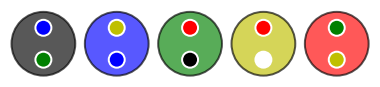
\includegraphics[scale= 0.45]{content/algo_selection/example/002.png}

		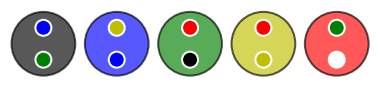
\includegraphics[scale= 0.45]{content/algo_selection/example/003.png}
		
		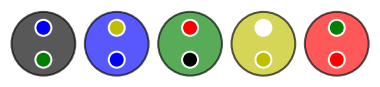
\includegraphics[scale= 0.45]{content/algo_selection/example/004.png}

		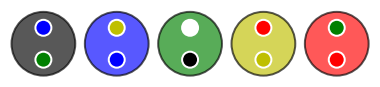
\includegraphics[scale= 0.45]{content/algo_selection/example/005.png}

		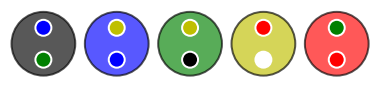
\includegraphics[scale= 0.45]{content/algo_selection/example/006.png}

		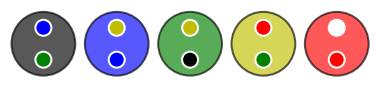
\includegraphics[scale= 0.45]{content/algo_selection/example/007.png}
	\end{center}
		
	\columnbreak
	\begin{center}
		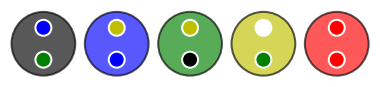
\includegraphics[scale= 0.45]{content/algo_selection/example/008.png}
		
		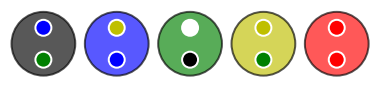
\includegraphics[scale= 0.45]{content/algo_selection/example/009.png}

		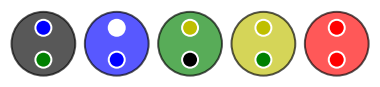
\includegraphics[scale= 0.45]{content/algo_selection/example/010.png}

		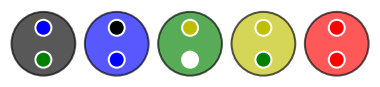
\includegraphics[scale= 0.45]{content/algo_selection/example/011.png}

		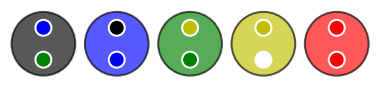
\includegraphics[scale= 0.45]{content/algo_selection/example/012.png}

		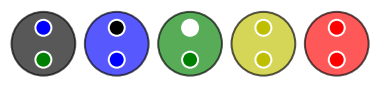
\includegraphics[scale= 0.45]{content/algo_selection/example/013.png}

		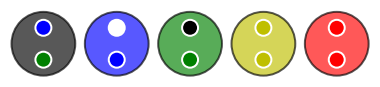
\includegraphics[scale= 0.45]{content/algo_selection/example/014.png}
			
		\textbf{\vdots}
		
		\textbf{etc}
	\end{center}
\end{multicols}


\medskip

Pour définir précisément comment fonctionne notre méthode, nous le faisons via l'algorithme suivant (l'écriture formelle employée est simple à comprendre).

\bigskip

\begin{algo}
	\Data{une configuration en ligne quelconque de début de jeu}
	\Result{une configuration en ligne où tous les jetons sont rentrées dans leur base}
	\vspace{0.4em}
    \Begin{
    	\vspace{0.4em}
		Aucune base n'est isolée pour le moment (nous allons vite voir ce que cela signifie).
    	\\
		\vspace{0.4em}
		\While{la configuration contient un jeton qui n'est pas dans sa base}{
			\vspace{0.4em}
			$\cal D$ : la base non remplie la plus à droite.
			\\
			$Coul_{\cal D}$ : la couleur de la base $\cal D$.
			\\
			\vspace{0.4em}
			\tcp{Les deux jetons de couleur $Coul_{\cal D}$ peuvent être dans la même base.}
			$j$ : un jeton de couleur $Coul_{\cal D}$ le plus à droite possible en dehors de la base $\cal D$. 
			\\
			$\cal J$ : la base du jeton $j$.
			\\
			\vspace{0.4em}
			\tcp{Deux contraintes.}
			$Ctr_1$ : ne pas passer par d'éventuelles bases isolées.
			\\
			$Ctr_2$ : ne pas bouger l'autre jeton de couleur $Coul_{\cal D}$ excepté si les deux jetons sont dans la même base.
			\\
			\vspace{0.4em}
			En respectant les deux contraintes $Ctr_1$ et $Ctr_2$,
			\\
			{\quad \textbullet} si besoin, amener le trou dans la base à droite de la base $\cal J$,
			\\
			{\quad \textbullet} puis utiliser le trou pour amener $j$ dans la base $\cal D$.
			\\
			\vspace{0.4em}
			\If{la base $\cal D$ est complète}{
				\vspace{0.4em}
				Isoler la base $\cal D$ (en la décalant un peu plus à droite par exemple). 
			}
        }
    }
\end{algo}

\bigskip

Nous devons vérifier la validité de cet algorithme c'est à dire vérifier trois choses.

\begin{enumerate}
	\item \textbf{\textsc{Non Ambiguïté :}} les actions proposées doivent être sans ambiguïté.

	\item \textbf{\textsc{Finitude :}} les actions à faire seront toujours en nombre fini.

	\item \textbf{\textsc{Résolution :}} une fois toutes les actions effectuées, nous devons obtenir une configuration où tous les jetons sont rentrées dans leur base.
\end{enumerate}


Le contrat de \quote{non ambiguïté} est rempli même si une certaine liberté est laissée pour déplacer le trou ou le jeton 
\footnote{
	Nous avons ici un bel exemple d'algorithme \quote{non déterministe} en ce sens qu'en lançant l'algorithme plusieurs fois sur la même configuration initiale, on ne passera pas forcément par les mêmes étapes intermédiaires pour résoudre le jeu.
}
à condition de ne pas visiter d'éventuelles bases isolées et sans bouger un éventuel jeton déjà bien placé dans la base la plus à droite non encore complète.
En pratique, la \quote{non ambiguïté} n'est jamais justifiée, par contre les deux derniers points doivent toujours faire l'objet d'une  démonstration comme nous allons le faire tout de suite.

\begin{proof}
	La preuve va s'appuyer sur deux résultats très simples dont on va donner des énoncés un peu formels mais avec des preuves visuelles très simples.


	\medskip

	\textit{Fait n°1 : on peut toujours déplacer le trou de la base où il est vers une base voisine $\cal V$ en laissant fixe un jeton de son choix dans la base $\cal V$.} 

	
	\medskip

	En effet, considérons le cas suivant où l'on veut déplacer le trou vers la troisième base en ne touchant pas au jeton rouge (les choix faits ne nuisent pas à la généralité du raisonnement pour un déplacement vers la droite).

	\vspace{-0.4em}
	\begin{center}   % [1, 2, 3, None, 4, 1, 4, 0, 2, 3]
		\includegraphics[scale= 0.45]{content/algo_selection/fact_1/000.png}
	\end{center}
	\vspace{-0.8em}

	Il suffit de procéder comme suit (c'est évident).

	\vspace{-0.4em}
	\begin{center}   % [2, 2, 3, None, 3, 1, 4, 0, 4, 1]
		\includegraphics[scale= 0.45]{content/algo_selection/fact_1/001.png}
	\end{center}
	\vspace{-0.8em}

	Le cas où la base voisine est à gauche se traite de façon analogue (on peut aussi utiliser un argument de type \quote{symétrie}).


	\medskip

	\textit{Fait n°2 : avec les notations de l'algorithme, on suppose le trou être dans la base ${\cal J}_d$ à droite de la base $\cal J$ du jeton $j$ à déplacer, et que cette base ${\cal J}_d$ n'est pas la base $\cal D$ à remplir. Dans ce cas, on peut placer le jeton $j$ dans la base ${\cal J}_d$ et le trou dans la base à droite de ${\cal J}_d$ en choisissant la place du trou.}

	
	\medskip

	La preuve est bien plus simple à comprendre que l'affreux énoncé ci-dessus (on se demande bien qui a pu rédiger un truc pareil). Ci-dessous, le jeton à déplacer est le jaune dans la deuxième base bleue, et nous choisissons de ne pas toucher au jeton jaune de la quatrième base jaune (le lecteur notera la généralité de la méthode proposée).

	\vspace{-0.4em}
	\begin{center}   % [1, 2, 3, 1, None, 0, 3, 2, 4, 4]
		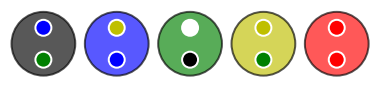
\includegraphics[scale= 0.45]{content/algo_selection/fact_2/000.png}

		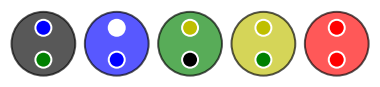
\includegraphics[scale= 0.45]{content/algo_selection/fact_2/001.png}

		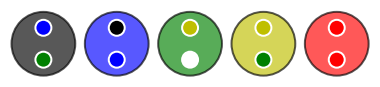
\includegraphics[scale= 0.45]{content/algo_selection/fact_2/002.png}

		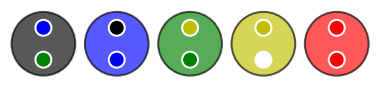
\includegraphics[scale= 0.45]{content/algo_selection/fact_2/003.png}

	\end{center}

	\vspace{-0.8em}


	\medskip

	\textit{Finitude et résolution} : commençons pas démontrer que l'algorithme commence par remplir la base rouge la plus à droite.


	\medskip

	Si la base rouge est déjà remplie, aucune action n'est requise et le résultat est vrai.
	Supposons donc que nous ayons au moins un jeton rouge dans l'une des quatre premières bases. Nous pouvons alors suivre les instructions de l'algorithme comme suit.


	\medskip

	\begin{itemize}
		\item[\textbullet] Grâce au fait n°1, il est effectivement possible de placer le trou dans la base à droite de celle du jeton rouge à déplacer, et ceci sans faire bouger un éventuel jeton rouge déjà dans la base rouge.

		\medskip

		\item[\textbullet] Ensuite, le fait n°2 nous permet d'amener le jeton rouge à déplacer dans l'avant-dernière base jaune et le trou dans la base rouge, de nouveau sans faire bouger un éventuel jeton rouge déjà dans la base rouge.

		\medskip

		\item[\textbullet] Il ne reste plus qu'à déplacer notre jeton rouge à la place du trou.
	\end{itemize}


	\medskip

	Si avant de faire ces opérations la base rouge contenait déjà un jeton rouge, nous avons rempli cette base, sinon l'algorithme nous fera remplir cette base dans un second temps (lors de la prochaine boucle \verb+Tant Que+).


	\medskip

	Une fois la base rouge remplie, celle-ci est isolée. Ceci implique que l'algorithme va travailler sur une version à quatre bases du jeu. Pour conclure, il suffit de reprendre le raisonnement ci-dessus non plus avec la base rouge mais avec la base jaune. Puis ensuite l'algorithme travaillera avec trois puis enfin deux bases et l'on raisonnera à chaque fois de la même façon. Ceci achève de montrer les propriétés de finitude et de résolution.

\end{proof}


\paragraph{Remarque :} \hspace{-1em} vous noterez que la démonstration précédente est valable pour un nombre quelconque $n \geqslant 2$ de bases (les plus tatillons pourront faire un raisonnement par récurrence).
